\chapter{Erstellung von Kookkurrenzgraphen}

Das folgende Kapitel beschreibt detailliert die Erstellung von Kookkurrenzgraphen. Dabei werden die Grundprinzipien erläutert, die existierenden Ähnlichkeitsmaße diskutiert und die algorithmische Umsetzung mittels MapReduce dargestellt.

\section{Grundprinzipien}

Um gewichtete inhaltliche Beziehungen zwischen Wörtern und Wortgruppen herstellen zu können, wird eine Definition von \emph{Ähnlichkeit} benötigt. Diese lässt sich auf vielfältige Arten bestimmen.

Die Ähnlichkeit zwischen zwei Dokumenten kann grundsätzlich nach \textcite{at1977} definiert werden. Dieser Definition liegt zu Grunde, dass sich die Dokumente als Mengen von Eigenschaften beschreiben lassen. Im Gegensatz zu anderen Ähnlichkeitsmodellen hängt die Ähnlichkeit nicht nur von den gemeinsamen Eigenschaften der Dokumente ab, sondern auch von den Eigenschaften, die die Dokumente allein besitzen. Diese Definiton von Ähnlichkeit wird in Abbildung \ref{fig:similarity} veranschaulicht.

\begin{figure}
\centering
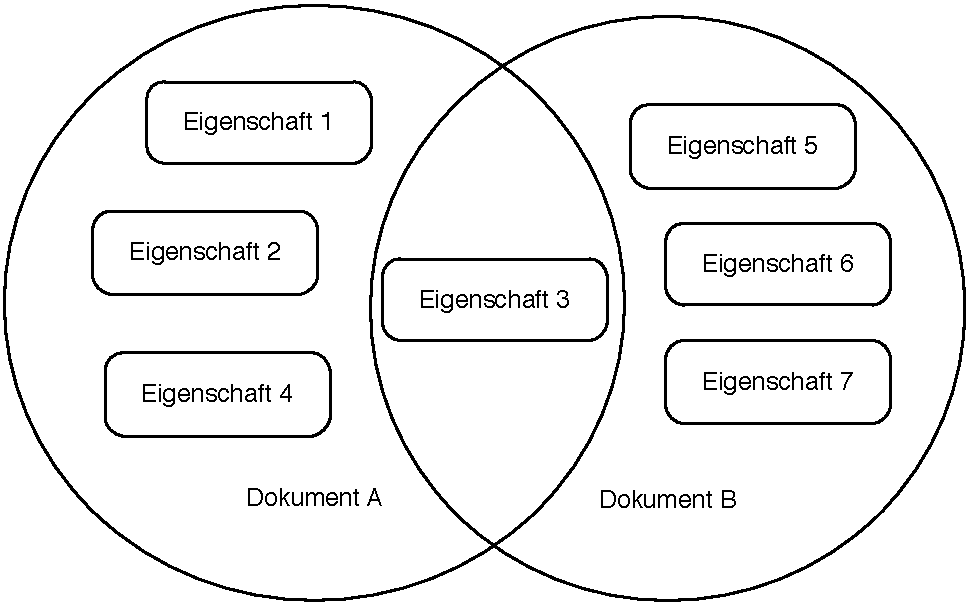
\includegraphics[width=0.8\textwidth]{similarity}
\caption{Repräsentation von Dokumenten als Mengen von Eigenschaften}
\label{fig:similarity}
\end{figure}

Somit lässt sich Ähnlichkeit \(s(A,B)\) zwischen den Dokumenten, die durch die Mengen \(A\) und \(B\) dargestellt werden, folgendermaßen definieren:
\[s(A,B) = F(A \cap B, A-B, B-A)\]
\label{similarity}

Die Gestaltung der Funktion \(s\) und die Auswahl der für die Ähnlichkeitsberechnung genutzten Eigenschaften der Dokumente hängt stark von der Anwendung ab. Somit beschreibt beispielsweise die Levenshtein-Distanz \cite{vl1966} die Ähnlichkeit zweier Zwichenketten durch die minmale Menge von Einfüge-, Lösch- und Ersetzungsoperartionen, die nötig sind, um eine Zeichenkette in die andere umzuwandeln. In Ontologien und Taxonomien kann die Ähnlichkeit von Begriffen mittels der Knoten- oder Kanteneigenschaften berechnet werden. Beispiele hierfür sind die Ähnlichkeit in Ontologien nach \textcite{pr1995} und \textcite{ps2002}. In der Bildverarbeitung können merkmalsbasierte Ähnlichkeitsmaße ebenfalls eingesetzt werden, beispielsweise beschreiben \textcite{ow2006} ein Ähnlichkeitsmaß auf Basis von Clusteringalgorithmen, die auf Rastergrafiken angewandt werden.

Im Kontext dieser Arbeit wird also ein Ähnlichkeitsmaß gesucht, dass anhand der Eigenschaften von Wörtern und Wortgruppen eine Distanz zwischen ebenjenen berechnet. Da eine inhaltliche Ähnlichkeit gesucht wird, spielen lingustische Ähnhlichkeitsmaße wie die Levenshtein-Distanz eine untergeordnete Rolle. Zu Beginn bestehen keinerlei Verbindungen zwischen den Zeichenketten, so dass keine Ähnlichkeitsmaße für Ontologien eingesetzt werden können.

Somit bietet sich die Wahl eines Ähnlichkeitsmaßes an, dass den Kontext, in dem die Wörter und Wortgruppen im Quellsystem verwednet werden, berücksichtigt.

\section{Kookkurrenz}

In \ref{data} wurden die für diese Arbeit verfügbaren internen Datenquellen beschrieben. Diese haben gemeinsam, dass zu den vorhandenen Wortgruppen nur wenig Kontext verfügbar ist. Im Falle des Tag-Systems ist bekannt, an welchen Dokumenten die Tags verwendet wurden. Das Clicktracking zeichnet die zu verwendeten Suchbegriffen geklickten Dokumente auf. Beide Datenquellen liefern also die Verwendungen von Wörtern und Wortgruppen zur inhaltlichen Beschreibung von Dokumenten.

Wenn mehrere Begriffe pro Dokument verwendet werden, wird damit ein Zusammenhang zwischen den Begriffen beschrieben. Dieser Zusammenhang lässt sich mit dem Ähnlichkeitsmaß \emph{Kookkurrenz} messen. Kookkurrenzmaße beschreiben, wie oft Begriffe gemeinsam verwendet werden. Dies wir dabei ins Verhältnis zum einzelnen Auftreten der Begriffe gesetzt und genügt somit der Definition von Ähnlichkeit in \ref{similarity}.

Dazu muss angemerkt werden, dass die Ähnlichkeit mittels Kookkurrenz nicht zwingend eine Ähnlichkeit der den Begriffen zu Grunde liegenden Konzepte darstellt. Die Verwendung von Kookkurrenz als Ähnlichkeitsmaß beruht allein auf der Annahme, dass Menschen zur Beschreibung von gleichen Inhalten die gleichen begriffe benutzen. Diese Annahme muss im Laufe der Evaluation der Ergebnisse validiert werden.

\section{Kookkurrenzmaße}
\label{measures}

Werden die Objekte, zwischen denen die Ähnlichkeit berechnet werden soll, als Mengen von Eigenschaften definiert, bieten sich die üblichen Kennzahlen für die Ähnlichkeiten von Mengen an. Ein Begriff kann also als Menge der Dokumente, für die er als Beschreibung verwendet wurde, definiert werden.

Um die Ähnlichkeit zwischen zwei Begriffen zu ermitteln, lassen sich die Vereinigungsmenge, Schnittmenge und Kreuzprodukte der jeweiligen Mengen bilden, die die Begriffe repräsentieren. Ist also \(A\) die Menge der Dokumente, die mit einem Begriff \(a\) versehen wurden, \(B\) die Menge der Dokumente mit einem Begriff \(b\), so ergeben sich die Mengen:

\begin{itemize}
    \item \(A \cap B\), alle Dokumente die mit \(a\) und \(b\) versehen wurden
    \item \(A \cup B\), alle Dokumente die mit \(a\) oder \(b\) versehen wurden
    \item \(A \times B\), alle Dokumentenpaare, die sich aus den Mengen \(A\) und \(B\) bilden lassen
\end{itemize}

Die Mächtigkeiten dieser Mengen können dann zur Berechnung verschiedener Ähnlichkeitsmaße verwendet werden. Drei der üblichsten Maße wurden im Rahmen dieser Arbeit verwendet und werden im folgenden genannt.

\subsection{Sørensen-Dice}

Der Sørensen-Dice-Koeffizient \cite{st1948} \cite{ld1945}, oft auch nur Dice-Koeffizient, stammt ursprünglich aus der Biologie und wurde verwendet, um die Ähnlichkeit zwischen Proben zu berechnen. Heute findet er allgemeine Anwendung im Data Mining. Er ist definiert durch:

\[
\delta_{Dice}(a, b) = \frac{2|A \cap B|}{|A|+|B|}
\]

Der Wertebereich des Koeffizienten liegt zwischen \num{0} und \num{1}.

\subsection{Jaccard}

Der Jaccard-Index \cite{pj19012} wurde ursprünglich mit dem gleichen Zweck wie der Dice-Koeffizient verwendet. Sein Wertebereich liegt ebenfalls zwischen \num{0} und \num{1} und er ist definiert durch:

\[
\delta_{Jaccard}(a,b) = \frac{|A \cap B|}{|A \cup B|}
\]

\subsection{Kosinus}

Die Kosinus-Ähnlichkeit \cite{hkp2012} ist ursprünglich ein Maß für die Ähnlichkeit zweier Vektoren. Sie ist eine Maßzahl dafür, ob die Vektoren ungefähr in die gleiche Richtung zeigen. Sie kann jedoch genauso auf Mengen angewendet werden, da das Vorhandensein der Elemente in der Menge auch durch einen Vektor in einem \(n\)-dimensionalen Raum dargestellt werden kann, wobei \(n\) die Anzahl aller möglichen Eigenschaften ist. Der Wertebereich der Kosinus-Ähnlichkeit liegt ebenfalls zwischen \num{0} und \num{1}. Sie ist auf den in \ref{measures} definierten Mengen folgendermaßen definiert:

\[
\delta_{Cosine}(a, b) = \frac{|A \cap B|}{\sqrt{|A| \times |B|}}
\]

Nachdem die Ähnlichkeit mittels Kookkurrenz und die entsprechenden Maße vorgestellt wurden, wird im nächsten Abschnitt die technische Umsetzung der Kookkurenzberechnung diskutiert.

\section{Umsetzung}

Im folgenden Abschnitt wird die Erstellung eines Graphen beschrieben, der die Kookkurrenzmaße für alle Paare von Begriffen enthält. Die Knoten stellen in diesem Fall die Begriffe dar. Die Kanten repräsentieren eine Kookkurrenz dieser Begriffe und werden mit den gewünschten Kookkurrenzmaßen annotiert. Existiert keine Kante zwischen zwei Knoten, so beträgt die Kookkurrenz zwischen den beiden repräsentierten Begriffen \num{0}.

Der Aufwand, um diesen Graphen zu erstellen, hängt also von der Anzahl der Begriffe, Dokumente, und Verbindungen von Begriffen und Dokumenten ab.

Für jedes Dokument muss, um die Ähnlichkeitsmaße zu berechnen, das Kreuzprodukt aller vergebenen Begriffe gebildet werden. Dabei muss das Auftreten jeder Paarung gezählt werden, um die Mächtigkeit der Menge \(A \cap B\) bestimmen zu können. Außerdem muss gezählt werden, wie oft jeder Begriff insgesamt verwendet werden, um die Mächtigkeit der Mengen \(A\), \(B\) usw. zu bestimmen. Beträgt die Anzahl der Begriffe \(n\) und die Anzahl der Dokument \(d\), so ergibt sich für den Fall, dass jeder Begriff an jedes Dokument vergeben wurde eine Laufzeit von \(O(d*n^2)\). Wurden keine Begriffe mit Dokumenten verknüpft, beträgt die Laufzeit \(\Theta(d)\). Die reale Laufzeit der Ähnlichkeitsberechnung daher liegt zwischen diesen Schranken.

Es ist also absehbar, dass der Rechenaufwand mit wachsender Datenmenge stark ansteigt. Somit scheint es ratsam, nach Optimierungen zu suchen, um die Rechenzeit zu verringern. Da sich die Anzahl der Berechnungen nicht vermindern lässt, kann eine Verkürzung der Rechenzeit nur durch Parallelisierung erreicht werden.

Da das Problem der Ähnlichkeitsberechnung nur lokale Berechnungen verwendet, ist eine Parallelisierung mittels des MapReduce-Programmiermodelles sinnvoll.

\subsection{MapReduce}
\label{mapreduce}

MapReduce \cite{dg2004} ist ein Programmiermodell für nebenläufige Verarbeitung und Erzeugung großer Datenmengen. Der Grundgedanke dieses Modells besteht in der Zerlegung der Berechnung in zwei Funktionen: \emph{Map} und \emph{Reduce}. Die Ein- und Ausgabedaten sind dabei Schlüssel-/Wertpaare. Beide Funktionen werden vom Benutzer spezifiziert.

Die Map-Funktion dient zur Erzeugung von Zwischenergebnissen, ebenfalls in der Form von Schlüssel-/Wertpaaren. Die Funktion wird dabei einzeln auf jedes Paar der Eingabedaten angewandt und kann eine beliebige Anzahl von Zwischenergebnissen \emph{emittieren}. Die MapReduce-Bibliothek gruppiert daraufhin alle Paare mit dem gleichen Schlüssel und übergibt diese an die Reduce-Funktion.

Die Reduce-Funktion wird also jeweils auf einen Schlüssel und eine Liste von Werten angewandt. Ziel dieser Funktion ist, für jeden Schlüssel kein oder ein Ergebnis zurückzugeben. Dabei werden die zu reduzierenden Werte für gewöhnlich als Iterator übergeben, um auch Datenmengen verarbeiten zu können, die nicht in den Arbeitsspeicher des Rechenknotens passen. Die Reduce-Funktion wird nur angewandt, wenn nach dem Map-Schritt mehr als ein Wert für einen Schlüssel emittiert wurde. Somit sollten Map- und Reduce-Funktion das gleiche Ausgabeformat besitzen. Das grundsätzliche Vorgehen von MapReduce ist in Abbildung \ref{fig:mapreduce} abgebildet.

\begin{figure}
\centering
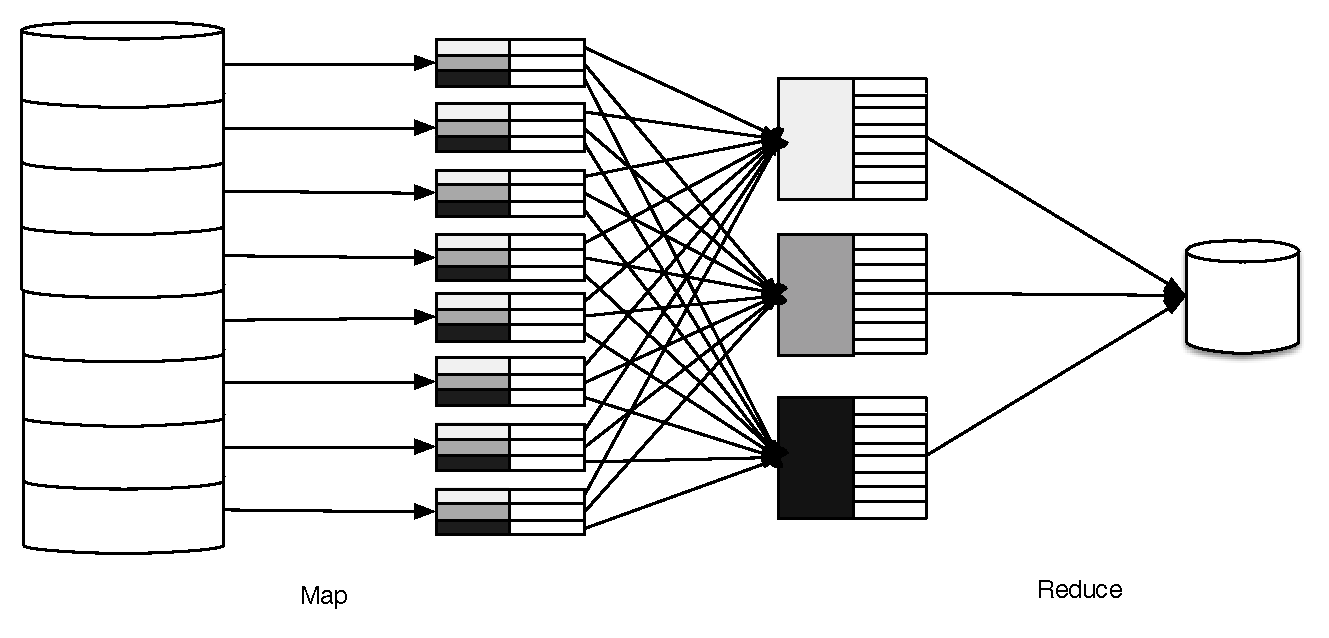
\includegraphics[width=\textwidth]{mapreduce}
\caption{MapReduce-Prozess}
\label{fig:mapreduce}
\end{figure}

Die MapReduce-Bibliothek übernimmt dabei sämtliche Kommunkation zwischen den Knoten des Rechnerclusters. Dies hat den Vorteil, dass der Programmierer nur über die Umwandlung des zu lösenden Problems auf das Programmiermodell, nicht aber um dessen Implementierung über mehrere Rechner hinweg kümmern muss. Somit kann die verwendete Hardware vergleichsweise einfach an die zu verarbeitende Datenmenge oder die Bedürfnisse an die Rechengeschwindigkeit angepasst werden.

In dieser Arbeit wurde die MapReduce Implementierung von MongoDB eingesetzt (siehe \ref{mongo}). Nach dieser grundsätzlichen Betrachtung des Programmiermodells wird im näachsten Abschnitt die Anwendung zur Berechnung von Kookkurenzen diskutiert.

\subsection{Anwendung von MapReduce}
\label{mapreduce_cooccurence}

MapReduce kann für die Berechnung der Knoten und Kanten des Kookkurrenzgraphen genutzt werden. Dazu müss für beide Operationen das Ein- und Ausgabeformat sowie die Funktionen Map und Reduce definiert werden.

Um die Berechnung zu vereinfachen, werden zuerst die Knoten erzeugt und mit allen Vorkommen der Begriffe annotiert. Somit kann daraufhin direkt aus der Knotenmenge die Kantenmenge erzeugt werden.

\subsubsection{Berechnung der Knoten}

Als Eingabedaten für die Berechnung der Knotenmenge dienen Tupel der Form \((d, t)\), wobei \(d\) ein Dokument und \(t\) einen Begriff darstellt. Die Map-Funktion wird nun auf jeden dieser Tupel angewandt und emmitiert Schlüssel-/Wertpaare mit dem Begriff als Schlüssel und einer einelementigen Liste, die das Dokument des Tupels enthält sowie der Zahl \num{1} als Anzahl Vorkommen dieses Begriffs. Dieses Vorgehen ist notwendig, da die Ausgabe der Map- und Reduce-Funktionen das gleiche Datenformat haben sollten.

Die Reduce-Funktion fasst die einelementigen Listen zusammen, addiert die Vorkommen und erzeugt somit den Knoten, der für einen Begriff alle Dokumente, die mit diesem Begriff versehen wurden, sowie die Anzahl der Vorkommen insgesamt enthält.

Die Map- und Reduce-Funktionen für die Knotenberechnung sind in Listings \ref{lst:mapred_nodes} als Pseudocode dargestellt.

\begin{lstlisting}[language=pseudo, label={lst:mapred_nodes}, caption={Knotenerzeugung mit MapReduce}]

function map(document, term) {
    emit(term, {documents: [document], count: 1});
}

function reduce(term, values) {
    result = {documents: [], count: 0};
    foreach value in values do
        result.documents = concat(result.documents, value.documents);
        result.count = result.count + value.count;
    end
    return result;
}
\end{lstlisting}

\subsubsection{Berechnung der Kanten}

Die Berechnung der Kantenmenge kann mit den vorher berechneten Knoten als Eingabedaten erfolgen. Dabei wird die Berechnung in 2 Bearbeitungsschritte aufgeteilt. Zuerst werden die annotierten Knoten so umgeformt, dass zu einem Dokument alle vergebenen Begriffe bekannt sind. Im zweiten Schritt werden alle Paare von miteinander auftretenden Begriffen gebildet und die Ähnlichkeitsmaße berechnet.

Algorithmus \ref{lst:mapred_edges1} zeigt die Umformung der Knoten mittels MapReduce. Als Eingabe für die Map-Funktion dienen die Knoten. Diese werden so umgeformt, dass für jedes Dokument, dass am Knoten annotiert ist, ein neues Schlüssel-/Wertpaar emittiert wird. Die Reduce-Funktion fasst die emittierten Ergebnisse zusammen, sodass als Ergebnis alle Begriffe, die an ein Dokument vergeben wurde, gesammelt als Liste vorliegen.

\begin{lstlisting}[language=pseudo, label={lst:mapred_edges1}, caption={Umformung der Knoten mit MapReduce}]
function map(node) {
    foreach document in node.documents do
        emit(document, {terms: [node]});
    end
}

function reduce(term, values) {
    result = {terms: []};
    foreach value in values do
        result.terms = concat(result.terms, value.terms);
    end
    return result;
}
\end{lstlisting}

In Algorithmus \ref{lst:mapred_edges2} wird die Erzeugung der Kookkurrenzkanten dargestellt. Im Map-Schritt werden dazu alle möglichen Paare der mit einem Dokument verknüpften Begriffe gebildet und emittiert. Der Schlüssel ist dabei eine Kombination aus Ziel- und Quellbegriff. Der Wert zählt die Anzahl der Kookkurrenzen zwischen beiden Begriffen. Im Reduce-Schritt werden alle Kanten zwischen zwei Termen zusammengefasst, die Summe der Kookkurrenzen gebildet und die Ähnlichkeitsmaße berechnet. Die Funktionen zur Berechnung der Maße sind in \ref{measures} beschrieben.

\begin{lstlisting}[language=pseudo, label={lst:mapred_edges2}, caption={Kantenerzeugung mit MapReduce}]
function map(document) {
    foreach term1 in document.terms do
        foreach term2 in document.terms do
            emit({source: term1, target: term2}, {count: 1});
        end
    end
}

function reduce(edge, values) {
    result = {count: 0, dice: 0, jaccard: 0, cosine: 0};
    foreach value in values do
        result.count = result.count + value.count;
    end
    result.dice = dice(edge.source, edge.target, result.count);
    result.jaccard = jaccard(edge.source, edge.target, result.count);
    result.cosine = cosine(edge.source, edge.target, result.count);
    return result;
}
\end{lstlisting}